\documentclass[oneside,12pt]{Classes/aesm_edspia}
\usepackage{minitoc}
\usepackage{float}
\usepackage{amsmath}
\usepackage{lmodern}%font modern
\rmfamily
\DeclareFontShape{T1}{lmr}{bx}{sc}{<->ssub * cmr/bx/sc}{} 
\usepackage{lettrine}
\usepackage{tabularx}
\usepackage{epsfig, floatflt, amssymb} 
\usepackage{moreverb} %% pour le verbatim en boite
\usepackage{cases}%equations en systemes numérotés - soluce possible package : CASES
\usepackage{multirow} %% pour regrouper un texte sur plusieurs lignes dans une table
\usepackage{url} %% pour citer les url par \url
\usepackage[all]{xy} %% pour la barre au dessus des symboles
\usepackage{textcomp} %% pour le symbol pour mille par \textperthousand et degrés par \degres
\usepackage[right]{eurosym}
\usepackage{setspace} %interligne simple, double etc...
\usepackage{Classes/eurosans} %%pour le symbole \euro
\usepackage{epic,eepic}
\usepackage{soul}
\usepackage[nottoc]{tocbibind} % tables des figures, des matieres et autres dans la TOC
\usepackage{fancybox}
\usepackage[leftcaption]{sidecap}
\usepackage[labelsep=endash, textfont={footnotesize, singlespacing}, margin=10pt, format=plain, labelfont=bf]{caption}
\usepackage[Conny]{Classes/fncychap} %en tete chapitrage
\newcommand{\ie}{c.-\`a-d.~}
\hbadness=10000% pb d'overfull box réglé
\hfuzz=50pt
\pdfcompresslevel9 % pour compresser le pdf final au maximum
\pdfoptionpdfminorversion=5 % pour accepté les images PDF version 1.5 (ex: celles produites par Office 2007)
\def\underscore{\char`\_}
\makeatletter
\renewcommand{\thesection}{\arabic {section}}
\renewcommand{\SC@figure@vpos}{c}% centrer verticalement le caption avec le package sidecap...
\renewcommand{\fnum@figure}{\small\textbf{Figure~\thefigure}}
\renewcommand{\fnum@table}{\small\textbf{Tableau~\thetable}}

\makeatother
\usepackage{subfig}
\def\thechapter{\Roman{chapter}}

%\usepackage[framed,numbered,autolinebreaks,useliterate]{Classes/mcode}


%%% Listings

\usepackage{listings}
\lstloadlanguages{xml, java}
	
	 \usepackage{listings}
  \usepackage{courier}
 \lstset{
         basicstyle=\footnotesize\ttfamily, 
         %numbers=left,               
         numberstyle=\tiny,          
         %stepnumber=2,               
         numbersep=5pt,              
         tabsize=2,                  
         extendedchars=true,         
         breaklines=true,            
         keywordstyle=\color[rgb]{0.43,0,0}\textbf,
    		frame=b,
         commentstyle=\color[rgb]{0.51,0.51,0.51} \textit ,
         stringstyle=\ttfamily  \color[rgb]{0,0.44,0} ,
         showspaces=false,           
         showtabs=false,             
         xleftmargin=17pt,
         framexleftmargin=17pt,
         framexrightmargin=5pt,
         framexbottommargin=4pt,
         %backgroundcolor=\color{lightgray},
         showstringspaces=false            
 }
 
 \usepackage{caption}
\DeclareCaptionFont{white}{\color{white}}
\DeclareCaptionFont{red}{\color{red}}
\DeclareCaptionFont{black}{\color{black}}
\DeclareCaptionFormat{listing}{\colorbox[cmyk]{0.43, 0.35, 0.35,0.01}{\parbox{\textwidth}{\hspace{15pt}#1#2#3}}}
\captionsetup[lstlisting]{format=listing,labelfont=black,textfont=white, singlelinecheck=false, margin=0pt, font={bf,footnotesize}}

\usepackage{float} % Required for [H] placement specifier
\usepackage{graphicx}
%%%%%%%%%%%%%%%%%%%%%%%%%%%%%%%%%%%%%%%%%%%
\begin{document}
%%%%%%%%%%%%%%%%%%%%%%%%%%%%%%%%%%%%%%%%%%%
\renewcommand\figurename{\small\textbf{Figure}} 

\addtocounter{page}{-1}%pour revenir à 0

% Pour remplir la page de garde

\TitreProjet{Object Detection Model : \\ Sign Language}

\AuteurA{Mariem} {Ksontini \vspace{22pt}}  
\AuteurC{Eya} {Ridene \vspace{20pt}}
\AuteurB{Sandra} {Mourali \vspace{20pt}}
%\AuteurD{Flen4} {FOULENI}

\Encadrant{Mr.}{Ahmed Baha}{Ben Jmaa}

%\EncadrantS{Dr.} {Rabaa} {Youssef}

\Filiere{Software Engineering}
%\datesout{09/01/2021}



% \President{Host Organization Supervisor} {Dr Sana Hamdi}     %% Président du Jury
% %\RapporteurA{Mme. Rapporteur} {FLENA} %%Rapporteur



\AnneeUniv{2022/2023}
% \begin{center} 
\includegraphics[scale=0.05]{insat.jpg} \end{center}

%%%%%%%%%%%%%%%%%%%%%%%%%%%%%%%%%%%%%%%%%%%

\makethese %% crée la couverture.
\onehalfspacing

\frontmatter %numérotation en iii
\pagestyle{fancy}
\fancyhf{}
\fancyfoot[R]{\thepage}
\renewcommand{\headrulewidth}{0.5pt}
\renewcommand{\footrulewidth}{0pt}
\renewcommand{\thesection}{\Roman{section}}
\renewcommand{\thesubsection}{\Roman{section}.\arabic{subsection}}
\renewcommand{\thesubsubsection}{\arabic{subsubsection}}

 

\begin{document}
%%%%%%%% TOC

%profondeur dans la table des matières et de la numérotation des sections

\setcounter{secnumdepth}{3}
\setcounter{tocdepth}{3}
\tableofcontents
\renewcommand\listfigurename{List of Figures}
\listoffigures \addcontentsline{toc}{List of Figures}

\renewcommand{\contentsname}%
    {Contents}%

%%%%minitoc
\dominitoc % génère la minitoc
\nomtcrule % supprime les lignes horizontales de la minitoc
\renewcommand{\mtctitle}{Plan} % Modifie le titre de la minitoc

%%%%


\renewcommand{\headrulewidth}{0.5pt}
\renewcommand{\footrulewidth}{0pt}
\fancyhead[R]{Object Detection Model}



\newpage % Start a new page
\hypertarget{1-abstract-}{%
\section{\texorpdfstring{\textbf{Abstract}}{Abstract}}\label{1-abstract-}}
The Personal Professional Project (PPP) project being carried out by the
National Institute of Applied Sciences and Technology (INSAT) includes
the production of this report. \\ Our project\textquotesingle s goal is to
create a hand gesture recognition model that can translate sign language
into spoken language in real time by utilizing the MediaPipe API. Our
PPP\textquotesingle s goal is to make it easier for hearing people to
communicate with deaf people by identifying the user\textquotesingle s
hand and facial movements and then converting those movements into words
or phrases.\\This will be accomplished by recognizing the
user\textquotesingle s hand and facial movements.
\vspace{10pt}

\begin{flushleft}
\textbf{\underline{Github Repository :}} \\
\url{https://github.com/mouralisandra/Sign-Language-Object-Detection}
\end{flushleft}


\vspace{50pt}

\hypertarget{2-introduction-}{%
\section{\texorpdfstring{\textbf{Introduction}}{Introduction}}\label{2-introduction-}}

The problem reigns in communication between those who have hearing
impairments and others who do not understand sign language which creates a barrier that inhibits deaf people from fully participating in everyday life. Taieb's personal experience with this topic, as the cousin of one of our teammates Sandra, has provided a moving picture of the dilemma. Taieb was born deaf and has battled his entire life to communicate with individuals who do not understand sign language. As a result of his struggles, he has developed a sorrowful condition. We were able to understand the importance of communication because of Taieb's example. Because only a small percentage of the population is competent in sign language, deaf people encounter challenges communicating with others and participating in many aspects of daily life.\\As a result, we concluded that designing a model for hand gesture detection would be the best strategy to assist Taieb and others in bridging the communication gap between hearing and deaf individuals. By recognizing hand and facial gestures and signals, we hope to be able to translate hand and face motions and signals into words or phrases.



\newpage % Start a new page
\hypertarget{3-the-goals-of-the-project}{%
\section{\texorpdfstring{\textbf{The Goals of The Project}}{The Goals of The Project}}\label{3-the-goals-of-the-project}}

\begin{itemize}
\item
  Design and build an object recognition model utilizing the MediaPipe API to discriminate hand and facial motions in a real-time video stream using landmarks; this model should be able to detect objects.
\item
  Make use of this model to transform the detected gestures into the matching letters of the sign language used by deaf individuals.
\item
  Using the webcam, display translations of motions captured by the camera on the screen.
\end{itemize}

If we are successful, communication between deaf and hearing people will evolve into a technique of personalized connection and exchange. This will give deaf people a voice while also encouraging greater understanding and empathy from society as a whole.


\vspace{5pt} % Add 10 points of vertical space
\hypertarget{4-methodology}{%
\section{\texorpdfstring{\textbf{Methodology}}{Methodology}}\label{4-methodology}}

To get started, we installed the necessary modules, which were Mediapipe, OpenCV, Pandas, NumPy, Scikit-learn, and TensorFlow. These modules enable the detection of poses, the processing of data, the encoding of labels, and the construction of models.

\hypertarget{41-the-accumulation-of-data}{%
\subsection{The Accumulation of
Data }\label{41-the-accumulation-of-data}}

\begin{itemize}
\item
  For this inquiry, we used Google and Pinterest, as well as other search engines, to find websites with images of people using sign language.
\item
  We thoroughly examined each photograph to ensure that our dataset was correct and accurate.
\item
  The gestures were meticulously documented, providing the model with translations that were both accurate and dependable for each move.
\item
  As a result, the titles of the photographs, links to the files where the images are saved, and labels that match to sign language motions are all included in our dataset, which was built using images obtained from the internet.
\item
  In addition, we used LabelEncoder to encrypt the labels before converting them to numbers.
\end{itemize}

\begin{figure}[h]
    \centering
    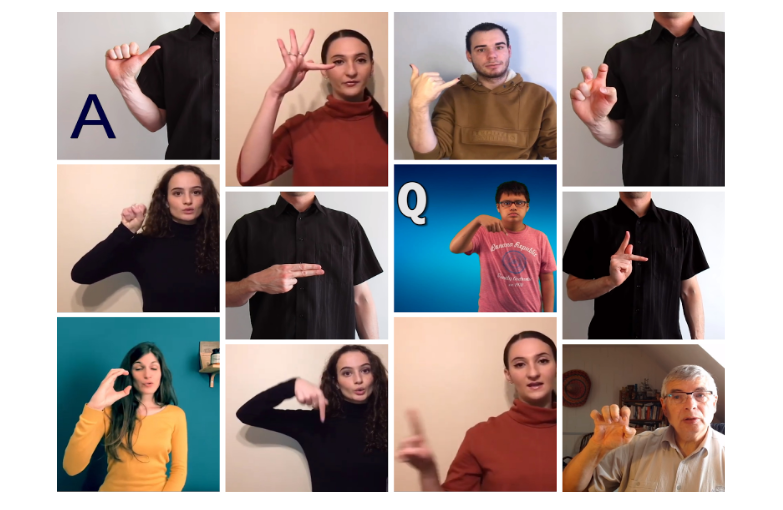
\includegraphics[width=0.9\linewidth]{Screenshot 2023-05-30 005658.png}
    \caption{A sample of images used in our dataset \vspace{10pt}}
\end{figure}
\vspace{50pt}

\begin{itemize}

\item 
  We traversed each image in the collection using
  Mediapipe\textquotesingle s hand detection capabilities to acquire the coordinates of the discovered hand landmarks.
\item
  We acquired the X, Y, and Z coordinate values for each hand point by adding these coordinates to the dataset.
\item
  The dataset was imported from a CSV file including the names of the photos, the paths to those images, and labels for the signs that comprise the French sign language alphabet.
\end{itemize}

\begin{itemize}
\item
  The \textquotesingle LabelEncoder\textquotesingle{} tool from scikit-learn is used to encode the sign labels into integers ranging from 0 to 25. \vspace{20pt}
  \end{itemize}

  \begin{figure}[h]
    \centering
  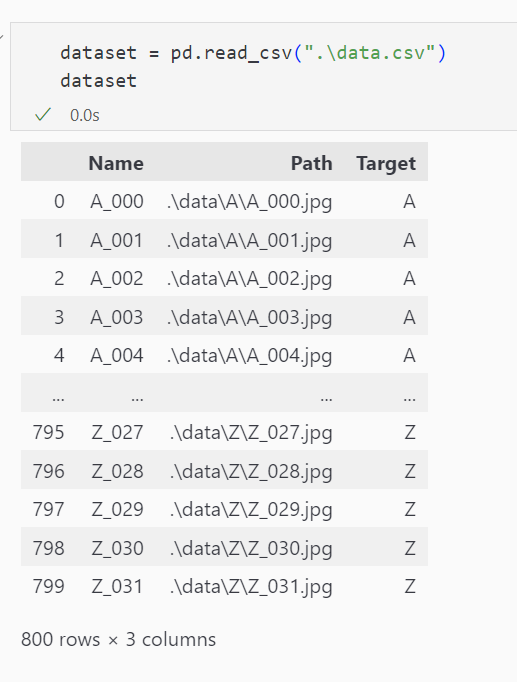
\includegraphics[width=0.5\linewidth]{Screenshot 2023-05-29 193143.png}
    \caption{The different instances of our dataset \vspace{10pt} }
\end{figure}


\hypertarget{42-data-preprocessing}{%
\subsection{Data Preprocessing }\label{42-data-preprocessing}}

\begin{itemize}
\item
  We subjected the data to a number of different preprocessing stages,
  one of which was the transformation of absolute coordinates into
  relative coordinates between the various hand points.
\item
  To do this, the X, Y, and Z values of each point were divided by the
  corresponding values of the wrist point.
\end{itemize}

\hypertarget{43-the-separation-of-the-data-into-training-and-test-sets}{%
\subsection{The Separation of The Data Into Training and Test Set : }\label{43-the-separation-of-the-data-into-training-and-test-sets}}


\begin{itemize}
\item
  We used the train\_test\_split function that is available in
  Scikit-learn to separate the data into a training set and a test set.
\item
  Because of this divide, we were able to isolate the data for both the
  training and the evaluation of the model.
\end{itemize}

\hypertarget{44-classification-models}{%
\subsection{Classification Models :}\label{44-classification-models}}

In order to classify the data for our research, we made use of two
different models : \\
Random Forest and an Artificial Neural Network (ANN).


\hypertarget{441-random-forest}{%
\paragraph{Random Forest}\label{441-random-forest}}

\begin{itemize}
\item
  With the help of the training data, we trained a Random Forest model.
  After that, we used the accuracy\_score function to determine the
  accuracy of the model by comparing our predictions to the data from
  the test set.
\item
  The Random Forest model\textquotesingle s performance was found to be
  about average, according to our findings.
\end{itemize}

\hypertarget{442-artificial-neural-network-often-referred-to-as-ann}{%
\paragraph{Artificial Neural Network (often referred to as
ANN)}\label{442-artificial-neural-network-often-referred-to-as-ann}}

\begin{itemize}
\item
  In addition to that, we used TensorFlow in the development of an ANN
  model. The model was trained using the training data and had several
  layers of densely packed data.
\item
  During the training phase, we made use of callbacks such as
  ReduceLROnPlateau and ModelCheckpoint in order to modify the learning
  rate and keep an eye on the model\textquotesingle s overall
  performance.
\item
  Following the training phase, we applied the model to the test set for
  evaluation and accuracy calculations.
\end{itemize}

\hypertarget{443-the-results-and-the-assessment}{%
\paragraph{The Results and the
Assessment}\label{443-the-results-and-the-assessment}}

\begin{itemize}
\item
  Following an analysis of both models, we came to the conclusion that
  the ANN model performed significantly better than the Random Forest
  model.
\item
  On the test set, the ANN model had an accuracy of 85\%, which
  indicates a reasonable capacity to classify sign language motions. \vspace{40pt}
\end{itemize}


\section{\textbf{Solution Architecture}}\label{5-solution-architecture}

\begin{figure}[H] % Use [H] instead of [h]
    \centering
    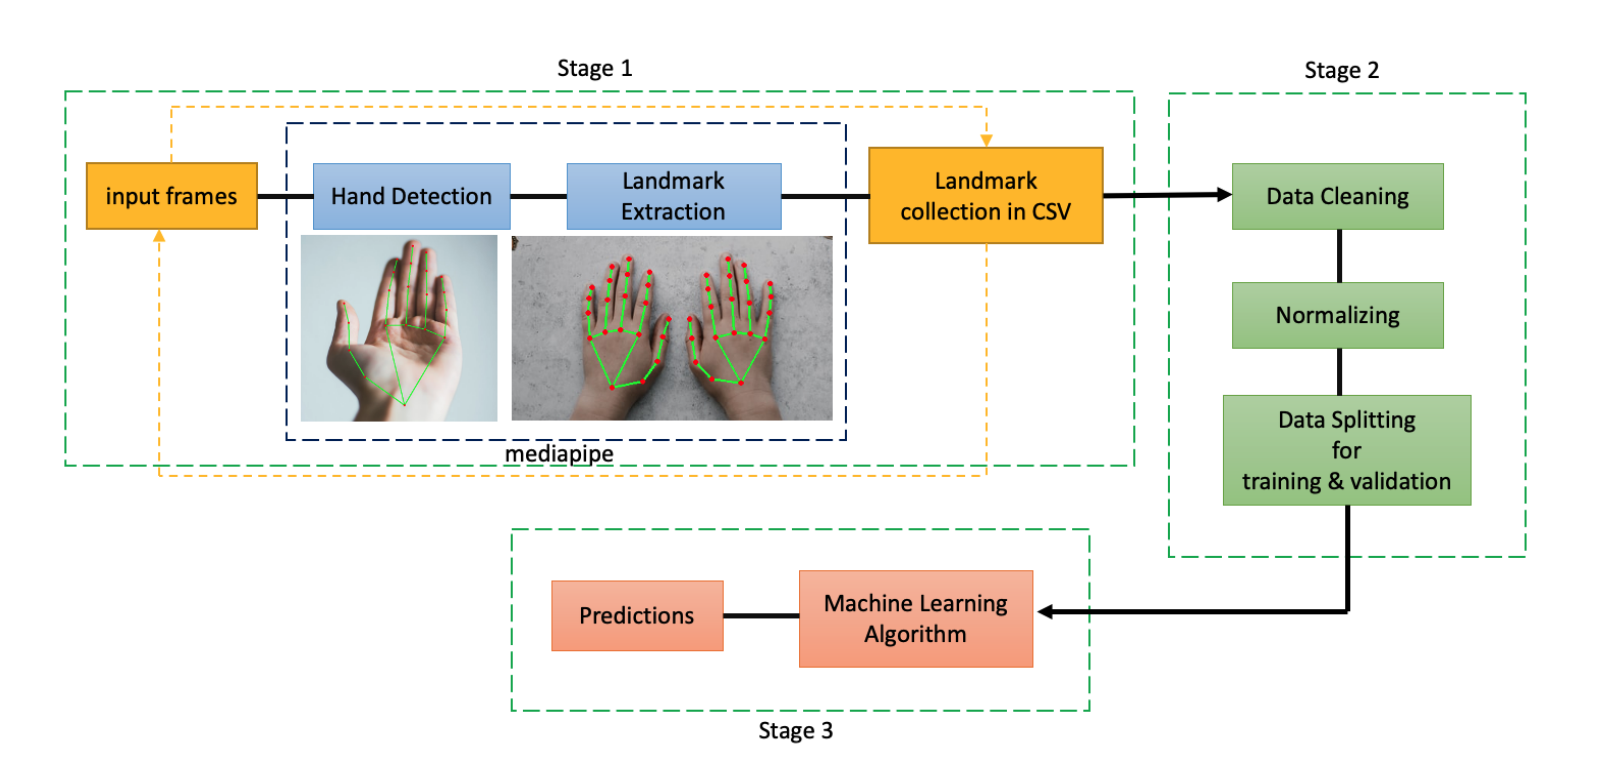
\includegraphics[width=1\linewidth]{Screenshot 2023-05-29 194320.png}
    \caption{Our Object Detection Model Architecture \vspace{10pt}}
\end{figure}
{\raggedright
This figure showcases the Proposed architecture to detect hand gestures and predict sign language finger-spelling. The suggested approach calls for the creation of a sign language classification system that makes use of hand position detection made possible via the Mediapipe API and classification made possible via the application of machine learning models.

\vspace{2\baselineskip} % Add two lines of vertical space

The process of classification is comprised of the following stages:
}


\hypertarget{stage-1-pre-processing-of-images-to-get-multi-hand-landmarks-using-mediapipe}{%
\subsection{Stage 1 : Pre-Processing of Images to get Multi-hand Landmarks using MediaPipe}\label{stage-1-pre-processing-of-images-to-get-multi-hand-landmarks-using-mediapipe}}

\hypertarget{configuration-of-the-components-of-the-mediapipe}{%
\subparagraph{Configuration of the Components of the
Mediapipe:}\label{configuration-of-the-components-of-the-mediapipe}}

\begin{itemize}
\item
  The configuration includes two Mediapipe
  components:\textquotesingle mp\_drawing\textquotesingle{} for
  displaying drawing detection results on the OpenCV screen
  and\textquotesingle mp\_holistic\textquotesingle{} for determining the
  hand posture.
\end{itemize}

\hypertarget{webcam-video-stream-retrieval}{%
\subparagraph{\texorpdfstring{ Webcam Video Stream
Retrieval:}{ Webcam Video Stream Retrieval:}}\label{webcam-video-stream-retrieval}}

\begin{itemize}
\item
  The OpenCV API is used to grab the video stream from the camera, and a
  loop is utilized to show the acquired video stream within an OpenCV
  window.
\end{itemize}

\hypertarget{pose-detection-of-the-hands}{%
\subparagraph{\texorpdfstring{ Pose Detection of the
Hands:}{ Pose Detection of the Hands:}}\label{pose-detection-of-the-hands}}

\begin{itemize}
\item
  The \textquotesingle mp\_holistic\textquotesingle{} component of
  Mediapipe is utilized so that hand pose detection may be carried out.
  Following the conversion of the video stream to RGB format, detection
  is carried out on each individual frame.\\
  The output includes both a display and a recording of the landmarks
  (points) of the hands that have been detected.
\end{itemize}

\hypertarget{real-time-prediction-of-the-sign}{%
\subparagraph{Real-time Prediction of the
Sign:}\label{real-time-prediction-of-the-sign}}

\begin{itemize}
\item
  Hand pose detection is carried out with the help of Mediapipe for each
  and every image that is taken from the camera.
\end{itemize}

\hypertarget{the-detection-of-hand-landmarks-and-the-extraction-of-coordinates}{%
\subparagraph{The Detection of Hand Landmarks and the Extraction of
Coordinates}\label{the-detection-of-hand-landmarks-and-the-extraction-of-coordinates}}

\begin{itemize}
\item
  We use Mediapipe\textquotesingle s hand detection functionality to run
  through all of the images in the dataset in order to retrieve the
  coordinates of the hand landmarks that are detected. After that, the
  landmark coordinates are changed into relative coordinates, which are
  used as features for the prediction.\\
  The MediaPipe documentation informs us that the coordinates of a
  detected hand are presented as follows:
  \begin{figure}[H] % Use [H] instead of [h]
    \centering
    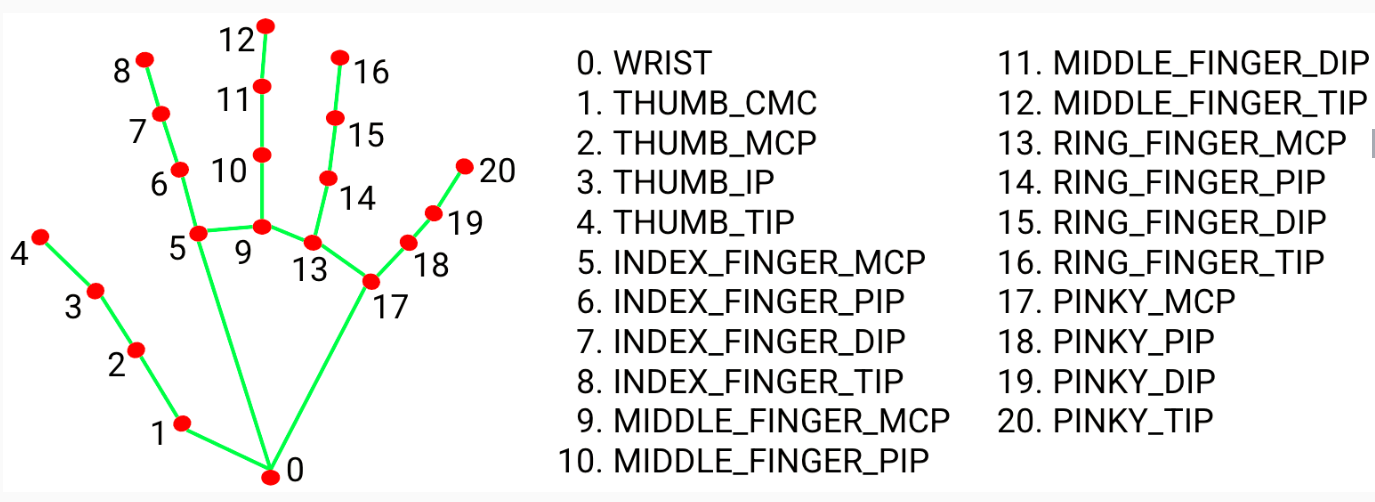
\includegraphics[width=0.9\linewidth]{Screenshot 2023-05-29 193440.png}
    \caption{ Hand Landmarks Detection \vspace{10pt}}
\end{figure}

\item
  Hence, the zero point corresponds to the wrist. It is using this point
  as a reference that we will convert absolute coordinates into relative
  coordinates.
\item
  To achieve this, we will divide the XYZ values of each point by the
  XYZ values of the wrist point.
\end{itemize}


\hypertarget{stage-2-data-cleaning-and-normalization}{%
\subsection{Stage 2 : Data cleaning and
normalization}\label{stage-2-data-cleaning-and-normalization}}


\hypertarget{detection-of-hands-in-dataset-photographs}{%
\subparagraph{Detection of Hands in Dataset
Photographs:}\label{detection-of-hands-in-dataset-photographs}}

\begin{itemize}
\item
  The photographs that are included in the dataset are loaded one at a
  time, and hand detection is carried out with the help of Mediapipe.
\item
  The X, Y, and Z coordinates of the landmarks on the hands that have
  been detected are saved in the dataset.
\end{itemize}

\hypertarget{the-initial-processing-of-data}{%
\subparagraph{The initial processing of
data:}\label{the-initial-processing-of-data}}

\begin{itemize}
\item
  In order to translate the absolute coordinates of the landmarks into
  their relative counterparts, the values are divided by those of the
  reference point, which in this case is the wrist.
\item
  The information is broken down into categories known as features (X)
  and labels (y).
\end{itemize}

\hypertarget{data-split}{%
\subparagraph{Data Split:}\label{data-split}}

\begin{itemize}
\item
  The \textquotesingle train\_test\_split\textquotesingle{} function
  found in scikit-learn is utilized in order to divide the data into a
  training set and a testing set.
\end{itemize}


\hypertarget{stage-3-prediction-using-machine-deep-learning-algorithm}{%
\subsection{Stage 3: Prediction using Machine/ Deep Learning Algorithm}\label{stage-3-prediction-using-machine-deep-learning-algorithm}}



\hypertarget{models-of-classification-}{%
\subparagraph{\texorpdfstring{ Models of Classification
:}{ Models of Classification :}}\label{models-of-classification-}}

\begin{itemize}
\item
  We make use of two different categorization models: Random Forest and
  an Artificial Neural Network (ANN) that is built on TensorFlow.
\item
  The ANN model is initially constructed with dense layers, then it is
  compiled with the Nadam optimizer and the
  "sparse\_categorical\_crossentropy" loss function, and finally, it is
  trained on the training set and validated using the test set.
\end{itemize}

\hypertarget{model-evaluation}{%
\subparagraph{Model Evaluation:}\label{model-evaluation}}

\begin{itemize}
\item
  The performances of the models are assessed by computing the
  prediction accuracy on the test set by employing the
  \textquotesingle accuracy\_score\textquotesingle{} function that is
  available in the scikit-learn library.
\end{itemize}

\hypertarget{data-classification}{%
\subparagraph{Data Classification}\label{data-classification}}

\begin{itemize}
\item
  In order to make an accurate prediction of the sign that corresponds
  to the hand coordinates, a trained classification model (either Random
  Forest or ANN) is utilized. This forecast is presented to the user on
  the screen right now.
\end{itemize}

\hypertarget{user-interface}{%
\subparagraph{User Interface:}\label{user-interface}}

\begin{itemize}
\item
  The findings of sign detection and prediction are displayed on a
  user-friendly interface that is designed to present the webcam video
  stream along with the results.
\item
  The user interface also enables people to engage with the system in
  various ways, such as the detection of starting and halting signs.
\item
  Following the selection and training of the object detection model, we
  incorporated it into the sign language translation application that we
  had developed. We took advantage of the MediaPipe framework, which
  provides powerful features for the capture and processing of real-time
  video streaming data.
\item
  This connection made it possible to identify hand and face movements
  in real time, producing rapid results that contributed to a fluid and
  responsive user experience.
\end{itemize}

\hypertarget{the-translation-of-gestures}{%
\subparagraph{The Translation of
Gestures}\label{the-translation-of-gestures}}

\begin{itemize}
\item
  After the accuracy of the gesture detection was confirmed, we went on
  to design a specific translation module. In order to identify
  different hand poses inside the webcam video stream, we made use of
  the Mediapipe API.
\item
  We were able to retrieve the coordinates of the hand landmarks that
  were detected by making use of Mediapipe\textquotesingle s detection
  components.
\end{itemize}

\hypertarget{translation-mapping}{%
\subparagraph{Translation Mapping}\label{translation-mapping}}

\begin{itemize}
\item
  We have added the translation functionality to the screen, which, when
  activated, shows a person who is deaf or hard of hearing the meaning
  of the movements they are making in real time when the gestures are
  recognized.
\item
  As a result, those who are deaf or hard of hearing will be able to
  communicate with one another regardless of language difficulties.
\end{itemize}
\vspace{50pt}

  \begin{figure}[H] % Use [H] instead of [h]
    \centering
    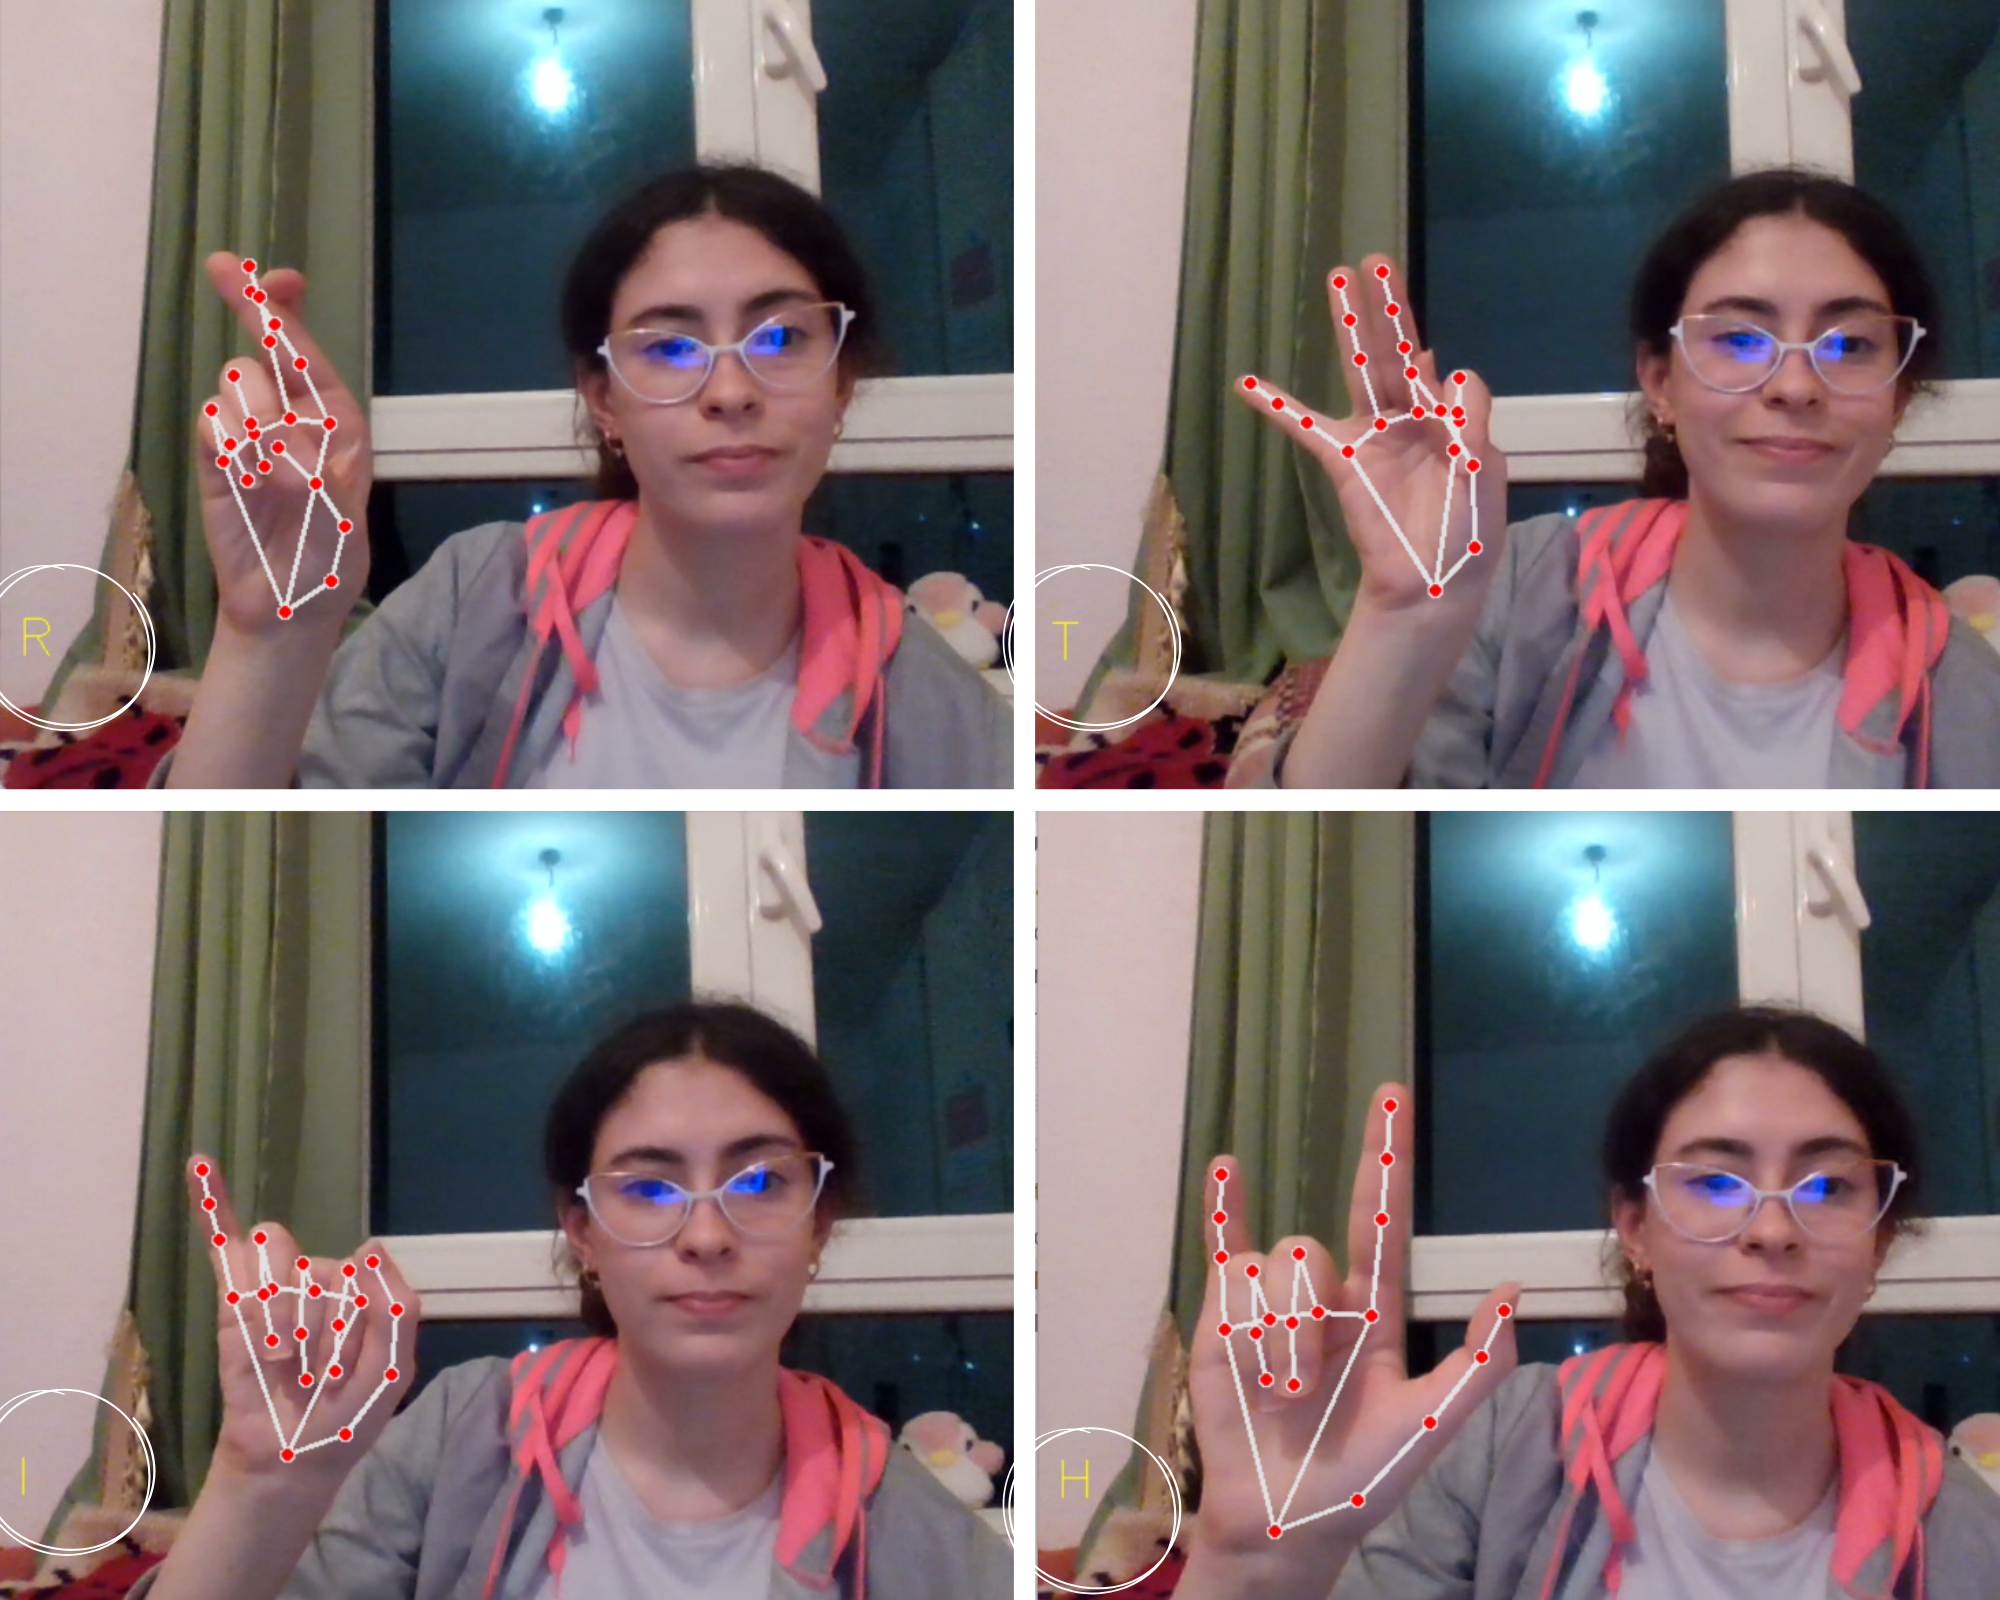
\includegraphics[width=0.9\linewidth]{Untitled design.png}
    \caption{ Testing The Translation Mapping \vspace{10pt} }
\end{figure}


\hypertarget{6-description-of-the-stringent-code}{%
\section{\texorpdfstring{\textbf{Description of The Stringent Code}}{Description of The Stringent Code }}\label{6-description-of-the-stringent-code}}

\begin{itemize}
\item
  The code that is going to be shown in this internship report is going
  to apply to the creation of a Sign Language categorization system that
  is going to use image databases that have been acquired from various
  sources on the internet such as Google, Pinterest, and other places.
\item
  In the first step of our process, we will import and perform any
  essential installs of modules that are necessary for our project. For
  the purposes of detection and computer vision, the mediapipe module
  together with its OpenCV dependency is installed on the system. In
  addition, we import modules for data manipulation, categorical data
  encoding, the development of machine learning models, and the training
  of deep learning models. These modules include pandas, numpy,
  scikit-learn, and tensorflow.
\item
  Next, we will configure two mediapipe components. The first is the
  drawing component, which will be used to display detection results on
  the OpenCV screen. The second is the holistic model, which will be
  used to identify hand pose.
\item
  Following that, we will utilize OpenCV to extract the video feed from
  the camera. In order to capture the video stream and display it in a
  window, we make use of a code snippet that is very simple.
\item
  Following this, we do hand posture detection tests using mediapipe on
  the video stream that was collected. We make use of the holistic model
  to determine the positions of the hands and present the landmarks
  (points) that are determined for each hand. To display the landmarks
  on the image that was captured, we make use of functions for drawing.
\item
  After ensuring that the hand detection system is operating as
  expected, we will go on to the next step of constructing a dataset. We
  import a CSV file that has information on the photos, the paths to
  those images, and the indicators that correspond to those images. We
  use LabelEncoder to encrypt the signs so that we may turn them into
  integers ranging from 0 to 25.
\item
  The next step is to identify any hands present in the dataset photos
  by utilizing mediapipe. We go over each image and pull out the
  landmarks of the hands that have been detected, then we add those
  landmarks to the dataset with their x, y, and z coordinates. There is
  a possibility that hands were not recognized in some of the
  photographs, therefore we skipped those and removed them from the
  dataset.
\item
  Following this, we divide each value by the corresponding values of
  the wrist point in order to convert the absolute coordinates of the
  landmarks into their relative coordinates. This brings the coordinates
  of the various hand points into a more consistent format.
\item
  Then, we used either the traditional train\_test\_split() method or
  StratifiedKFold to divide our data into training and testing sets.
  This was done to ensure that the proportions of each sign remained the
  same in both the training and testing sets.
\item
  After that, we will move on to the process of developing
  classification models and training them. To get started, we use the
  RandomForestClassifier class from the scikit-learn library to create a
  Random Forest model. While the model is being trained on the training
  set, its accuracy is being evaluated using the test set. We carry out
  the procedure once more while utilizing StratifiedKFold so that we may
  compare the outcomes.
\item
  Lastly, we investigate the possibility of using a neural network for
  the classification of signs. Using the Sequential function that is
  provided by Keras, we create an ANN model, also known as a dense
  neural network. In order to perform multiclass classification, we add
  dense layers that are activated by ReLU, as well as an output layer
  that is activated by softmax. When we are through setting the loss
  function, optimizer, and evaluation metrics, we will compile the
  model.
\item
  Following this, the ANN model is trained using the training set, and
  then its accuracy is evaluated using the test set. We present the
  results of the accuracy and loss measurements for each training epoch.
\end{itemize}
\newpage

\hypertarget{7-the-section-on-testing-and-evaluation-is-as-follows}{%
\section{\texorpdfstring{\textbf{Testing and Evaluation}}{Testing and Evaluation}}\label{7-the-section-on-testing-and-evaluation-is-as-follows}}

We used two different models---a Random Forest and an Artificial Neural
Network (ANN)---in order to evaluate the effectiveness of our system for
classifying French Sign Language signs.

\hypertarget{random-forest-model}{%
\subsection{Random Forest Model}\label{random-forest-model}}

\begin{center}
    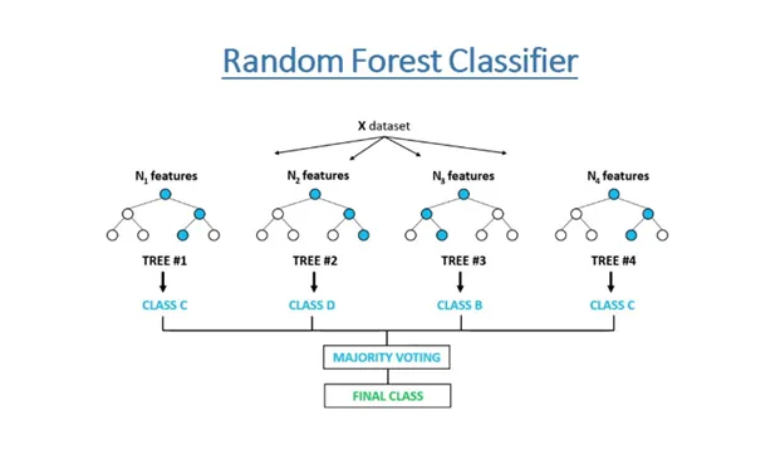
\includegraphics[width=1\linewidth]{Screenshot 2023-05-30 005426.png}
    \captionof{figure}{Random Forest Classifier \vspace{10pt}}
\end{center}



\vspace{20pt}
\begin{itemize}
\item
  With the help of the training data, we trained a Random Forest model.
  Following that, we produced predictions based on the test data and
  determined the accuracy of the model.
\item
  The Random Forest model provides an accuracy of 0.85 when applied to
  the test data.
\end{itemize}
\vspace{10pt}
\begin{center}
    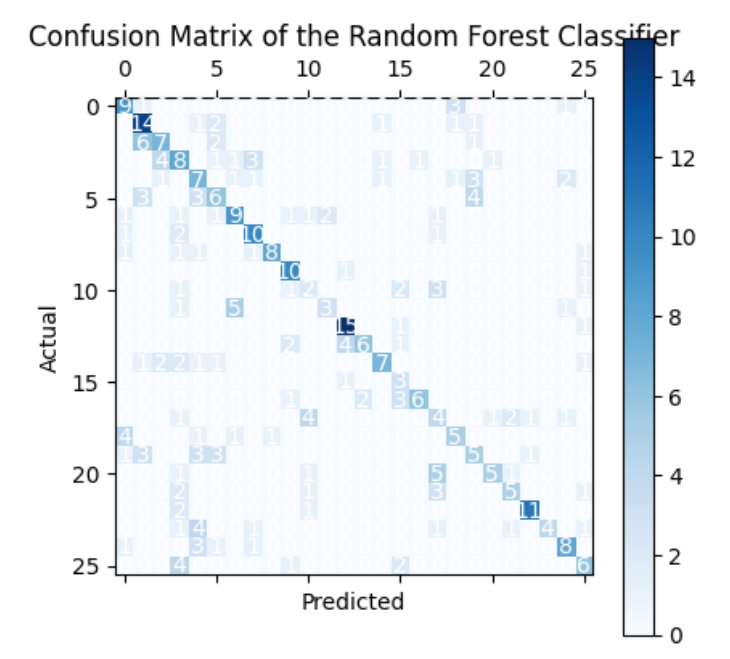
\includegraphics[width=0.7\linewidth]{randomForest.png}
    \captionof{figure}{Confusion Matrix of the Random Forest Classifier}
\end{center}

\hypertarget{ann-model}{%
\subsection{ANN Model}\label{ann-model}}


\begin{center}
    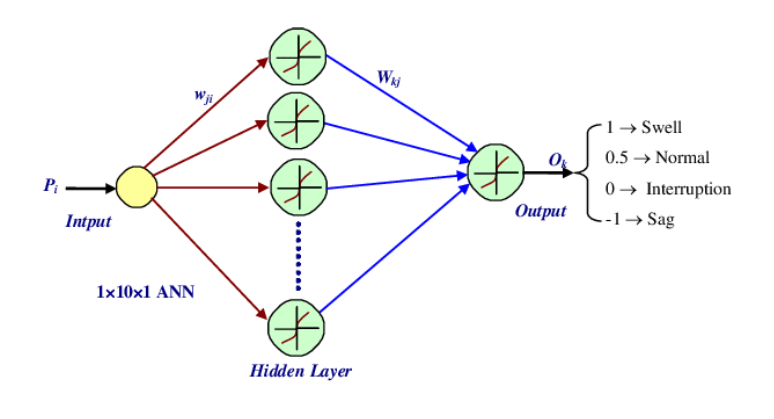
\includegraphics[width=0.9\linewidth]{Screenshot 2023-05-30 005441.png}
    \captionof{figure}{Artificial Neural Network Model (ANN Model)}
\end{center}

\vspace{20pt}

\begin{itemize}
\item
  In addition to that, we used the training data to train an ANN model.
  We made use of a multi-layered neural network that contained input
  layers, hidden layers, as well as an output layer. Compilation of the
  model was done using the Nadam optimizer and the
  "sparse\_categorical\_crossentropy" loss. We were able to slow down
  the rate of learning and preserve the weights of the model that
  performed the best thanks to callbacks.
\item
  In order to train the ANN model, XX epochs were used, and the batch
  size was also XX. We calculated the model\textquotesingle s accuracy
  using the test data in order to evaluate its performance.
\item
  On the basis of the test data, the ANN model has an accuracy of 0.92.

\end{itemize}
\vspace{10pt}

 \begin{center}
  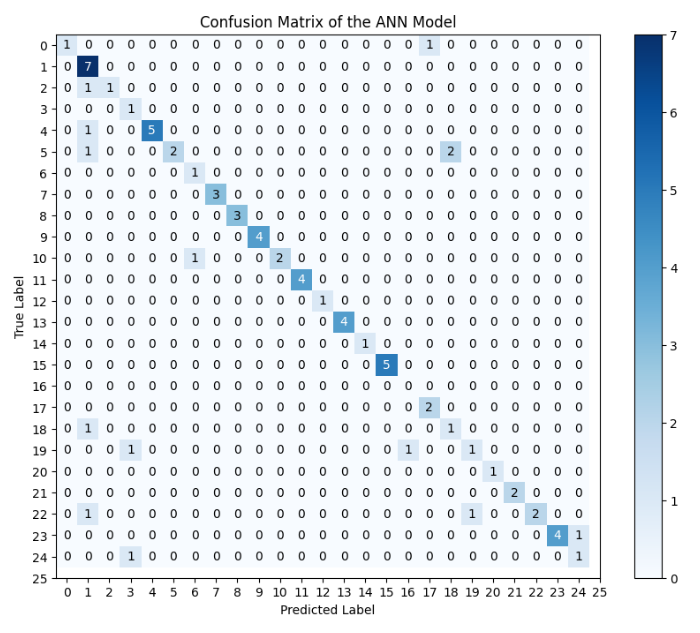
\includegraphics[width=0.8\linewidth]{ANNMatrix.png}
   \captionof{figure}{Confusion Matrix of the ANN Model \vspace{10pt} }
  \end{center}

\hypertarget{contrast-between-the-models}{%
\subsection{Contrast Between
Models}}{Contrast Between Models}\label{a-contrast-between-the-models}

\begin{itemize}
\item
  On the basis of the test data, it seems that the ANN model has a
  higher level of accuracy than the Random Forest model. This provides
  support for the notion that the ANN model is superior for the
  classification of French Sign Language signs.
\item
  Before coming to any conclusive conclusions regarding the
  models\textquotesingle{} performances in comparison to one another, it
  is advisable to carry out evaluations that are more in-depth and make
  a comparison of how well the models performed on several metrics.
\item
  It is also essential to stress that the performance of a
  classification model can be affected by other factors, like the size
  and quality of the dataset, the preprocessing techniques that are
  utilized, and the assessment metrics that are selected. Because of
  this, it is absolutely necessary to take these aspects into
  consideration and carry out exhaustive research in order to get an
  in-depth comprehension of the capabilities and restrictions exhibited
  by the models.
  \vspace{10pt}
  
  \begin{center}
  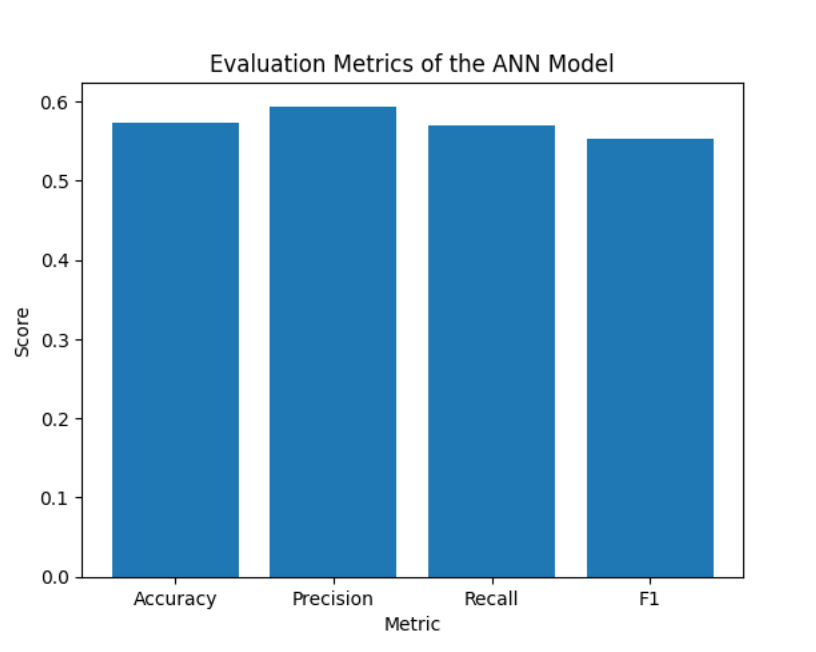
\includegraphics[width=0.8\linewidth]{Screenshot 2023-05-30 010022.png}
   \captionof{figure}{Evaluation Metrix of the ANN Model \vspace{10pt} }
  \end{center}
\item
  In conclusion, the results of our testing and evaluation reveal that
  our sign categorization system is effective. In particular, the ANN
  model demonstrates promising accuracy.
\item
  However, additional research and experimentation are strongly urged so
  that the system\textquotesingle s robustness can be improved and
  additional performance measures can be investigated.
\end{itemize}

\hypertarget{8-possible-enhancements}{%
\section{\texorpdfstring{\textbf{Possible Enhancements}}{Possible Enhancements}}\label{8-possible-enhancements}}

\begin{itemize}
\item
  Advanced deep learning methods, such as Convolutional Neural Networks
  (CNN), can be incorporated into the system to improve its ability to
  recognize hand poses and classify signs. This is one way to improve
  the system.
\item
  The potential for the system to become more adaptable and beneficial
  to users is increased with the addition of functions such as hand
  movement detection or sign translation into text or audio.
\item
  It is essential to emphasize the fact that the aforementioned
  description offers a high-level summary of the solution that has been
  suggested. The real implementation can call for some alterations and
  additional details to be worked out based on the particular
  specifications and prerequisites of the project.
\item
  Hand pose detection is carried out with the help of Mediapipe for
  every single image that is taken from the camera.
\end{itemize}

\vspace{200pt}
\hypertarget{9-conclusion}{%
\section{\texorpdfstring{\textbf{Conclusion}}{Conclusion}}\label{9-conclusion}}

\begin{itemize}
\item
  Using MediaPipe's technology and machine learning, our suggested technique shows that MediaPipe can accurately detect complicated hand gestures.
\item
  Sign language modeling utilizing image processing techniques has evolved over the years, but approaches are difficult and demand considerable computer capacity.
\item
  Model training is time-consuming. This study sheds light on the issue. The model is resilient and cost-effective due to less computer power and smart device flexibility.
\item
  Training and testing with diverse sign language datasets reveal this framework can be tailored to any regional dataset for optimal accuracy.
\item
   Faster real-time detection shows the model's efficiency. Mediapipe's top classification algorithms can be used to recognise sign language words from videos in the future.
\item
   We also plan to add data to strengthen our gesture database and broaden its indication coverage. To improve communication, we want to detect longer and more complex phrases and translate them into many languages. 
\item
  In conclusion, our goal is to remove barriers to communication for deaf and non-sign language users. We are committed to enhancing our system and contributing to a more inclusive society.
\end{itemize}

\newpage
\hypertarget{10-contribution-of-team-members}{%
\section{\texorpdfstring{\textbf{Contribution of Team Members}}{Contribution of Team Members}}\label{10-contribution-of-team-members}}

\hypertarget{mariem-ksontini}{%
\subsection{Mariem Ksontini}\label{mariem-ksontini}}

\begin{itemize}
    \item
    Collected data by scouring the internet for sign language photos, documenting them meticulously, and compiling the dataset.
    
    \item
    Used LabelEncoder to encrypt the sign language labels and convert them to numerical values.

    \item
    Used Mediapipe to seek and retrieve the coordinates of hand landmarks in photos for the hand detection capability.
    
    \item
    Aided in data preprocessing by converting absolute coordinates to relative coordinates.

\end{itemize} 

\hypertarget{eya-ridene}{%
\subsection{Eya Ridene}\label{eya-ridene}}


\begin{itemize}
    \item
    Worked on data preprocessing, such as converting absolute coordinates to relative coordinates between hand points.
    \item
    Used Scikit-learn's train test split function to divide the data into training and test sets.

    \item
    Helped to implement the Random Forest model for classification and evaluated its performance with the accuracy score function.
    
    \item
    Assisted in the analysis and comparison of the Random Forest model's findings with the ANN model.

\end{itemize} 

\hypertarget{sandra-mourali}{%
\subsection{Sandra Mourali}\label{sandra-mourali}}

\begin{itemize}
    \item
     Used TensorFlow to implement the Artificial Neural Network (ANN) model and train it with training data.

    \item
    Used to alter the learning rate and monitor the model's performance  during the training phase, callbacks such as ReduceLROnPlateau and ModelCheckpoint
    
    \item
    For evaluation, applied the trained ANN model to the test set and calculated the accuracy.

    \item
     Assisted in the performance analysis of the ANN model, which was determined to be much superior than the Random Forest model.
\end{itemize}

\hypertarget{collaborative-efforts}{%
\subsection{Collaborative Efforts}\label{collaborative-efforts}}

\begin{itemize}
    \item
    Worked together on overall approach design and problem-solving.

    \item
    Assisting with the interpretation and analysis of the results from both models.
    
    \item
    Helped develop the suggested solution architecture for recognizing hand motions and predicting sign language finger-spelling.
    
    \item
     Collaborated on integrating the models into an easy-to-use interface for real-time sign language translation.

     \item
     Worked on translation mapping and implementing translation features to help deaf and hard of hearing people communicate.

     
\end{itemize}

\setcounter{secnumdepth}{3}
\setcounter{tocdepth}{3}

\renewcommand{\contentsname}{References}

%%%%minitoc
\dominitoc % generates the minitoc
\nomtcrule % removes the horizontal lines from the minitoc
\renewcommand{\mtctitle}{Plan} % Modifies the title of the minitoc

%%%%
\begin{document}
\pagestyle{fancy}
\renewcommand{\headrulewidth}{0.5pt}
\renewcommand{\footrulewidth}{0pt}
\tableofcontents
\begin{itemize}
\item
  Mediapipe Documentation. Available online:
  \url{https://mediapipe.dev/}
\item
  OpenCV Documentation. Available online: \url{https://docs.opencv.org/}
\item
  Documentation pertaining to Pandas. Available online:
  \url{https://pandas.pydata.org/}
\item
  The documentation for NumPy. Available online:
  \url{https://numpy.org/doc/}
\item
  Documentation for the scikit-learn package. Available online:
  \url{https://scikit-learn.org/stable/documentation.html}
\item
  The documentation for TensorFlow. Available online:
  \url{https://www.tensorflow.org/api_docs}
\end{itemize}

\end{document}


\newpage % Start a new page
\hypertarget{references}{%
\subsection{References:}\label{references}}
\item
  Mediapipe Documentation. Available online:
  \url{https://mediapipe.dev/}
\item
  OpenCV Documentation. Available online: \url{https://docs.opencv.org/}
\item
  Documentation pertaining to Pandas. Available online:
  \url{https://pandas.pydata.org/}
\item
  The documentation for NumPy. Available online:
  \url{https://numpy.org/doc/}
\item
  Documentation for the scikit-learn package. Available online:
  \url{https://scikit-learn.org/stable/documentation.html}
\item
  The documentation for TensorFlow. Available online:
  \url{https://www.tensorflow.org/api_docs}
\end{itemize}





%%%%%%%% Figures

% \makeatletter
% %\renewcommand{a\thefigure}{\@arabic\c@figure}
% \@addtoreset{figure}{chapter}
% \makeatother

% \renewcommand{\headrulewidth}{0.5pt}
% \renewcommand{\footrulewidth}{0pt}
% \renewcommand\listfigurename{Figures List}
% \listoffigures \mtcaddchapter 

% \fancyhead[R]{Liste des Figures}
% \newpage

\makeatletter
     \renewcommand*\l@figure{\@dottedtocline{1}{1em}{3.2em}}
\@addtoreset{figure}{chapter}
\makeatother
\renewcommand{\headrulewidth}{0.5pt}
\renewcommand{\footrulewidth}{0pt}




%%%%%%%% Tableaux

\makeatletter

\renewcommand{\headrulewidth}{0.5pt}
\renewcommand{\footrulewidth}{0pt}
\renewcommand\listtablename{Tables List}

% \listoftables  \mtcaddchapter 

% \fancyhead[R]{Liste des Tableaux}

%%%%%%%%%%%%%%%%%%%%%%%%%%%%%%%%%%%
%%%%%%%%%%%%%%%%%%%%%%%%%%%%%%%%%%%




    % \documentclass[oneside,12pt]{Classes/aesm_edspia}
% \usepackage[utf8]{inputenc}
% \usepackage[LFE,LAE,OT1]{fontenc}

% \usepackage[french,english,arabic]{babel}

\pagestyle{fancy}

%\usepackage{graphicx}
\begin{document}
\setlength{\parindent}{0pt}
\setlength{\topmargin}{0mm}
\setlength{\headheight}{0cm} 
\setlength{\headsep}{0cm}
\setlength{\textheight}{20cm}
\setlength{\textwidth}{17cm} 
\setlength{\marginparsep}{0cm} 
\setlength{\marginparwidth}{0cm}
\setlength{\headheight}{0cm} 
\setlength{\footskip}{0cm}

\pagestyle{fancy}



\end{document}
\end{document}